\documentclass[10pt,a4paper,titlepage]{article}
\usepackage[utf8]{inputenc}

\usepackage{amsmath}
\usepackage{amsfonts}
\usepackage{amssymb}
\usepackage{graphicx}
\usepackage{float} % force figure to render inline location
\usepackage{enumitem} % apt install texlive-latex-extra 
\usepackage{anyfontsize} % custom fontsizes
\usepackage{titlesec} % custom section spacings
\usepackage{multirow} % merge table rows
\usepackage{vhistory} % revision table package
\usepackage{pdfpages}
\usepackage{wrapfig}
\usepackage{lscape}
\usepackage{rotating}
\usepackage{epstopdf}
\usepackage{caption}
\usepackage{subcaption}
\usepackage{nameref} % allows use of named references

\setlist[itemize]{noitemsep} % No spaces in itemize lists
\setlist[enumerate]{noitemsep} % No spaces in itemize lists
\setlist[description]{noitemsep} % No spaces in itemize lists
\titlespacing*{\subsubsection}{0pt}{8pt}{2pt}
\titlespacing*{\paragraph}{0pt}{3pt}{5pt}

\newcommand{\cpright}{\textsuperscript{\tiny\copyright}}

\setlength\parindent{0pt}

\begin{document}
	
	\begin{titlepage}
		
		\title{
			\fontsize{50}{12}\selectfont{\textsc{Lunar Rover}}\\
			\vspace{20pt}
			\fontsize{20}{12}\selectfont{\textsc{Testing Summary}}\\
			\vspace{10pt}
			\large{Software Engineering \& Project} \\
			\vspace{20pt}
			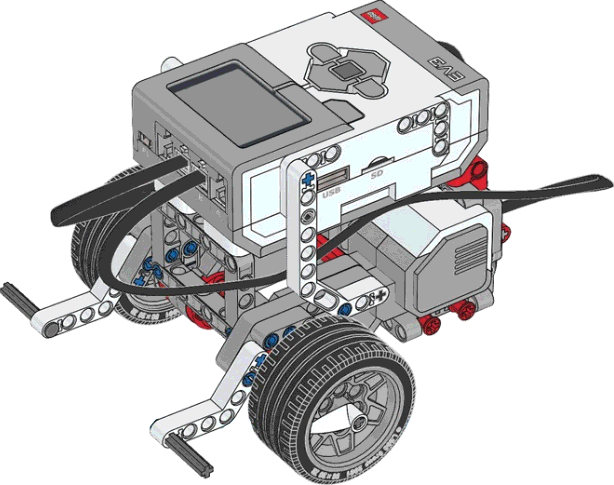
\includegraphics[width=200px]{title-page-ev3.png}					
		}
		\date{3/10/2017}
		\author{
			\bf{Team: PG-29} \\
			Kin Leong Lee \\
			Sean Hennessy
		}
		\maketitle
	\end{titlepage}
		 
	\tableofcontents	
	\listoftables
		
	\section*{Revision History}	
	\label{revtable}	
	\begin{tabular}{|p{2.1cm}|p{2.5cm}|p{2cm}|p{4.1cm}|}		
		\hline 
		\textbf {Name} & \textbf{Date} & \textbf {Version} &\textbf {Summary of Changes} \\ \hline
		Issac Lee & 25-Oct-2017 & 0.1 & Fixed some symbols display issue\\ \hline
		Sean & 27-Oct-2017 & 1.0 & Formatting and grammar, Final released\\ \hline	
	\end{tabular}

	\newpage	
	\section{Introduction}
		\subsection{Purpose}
		This Lunar Rover Test Report provides a summary of the results of test performed as outlined within this document. The software unit tests are running continuously thoroughly the development phases. The final acceptance test is running on 22-Oct-2017 and all type of tests will be running.
	
	\section{TEST SUMMARY}
\begin{itemize}
\item \textbf{Project Name:}  Lunar Rover
\item \textbf{System Name:} Michael Jackson
\item \textbf{Version Number:} 1.0
\end{itemize}
	\subsection{SOFTWARE UNIT TESTS}
	All unit tests are created by JUNIT and running on each development phase to ensure that the system can be running without any unexpected issue.
\subsubsection*{}
	\begin{itemize}
\item \textbf{Test Owner:}  Kin Leong Lee
\item \textbf{Test Date:}: 22-Sep-2017
\item \textbf{Test Description:} To test the Event system can reference the difference unit object
\item \textbf{Test Results:} PASS – All objects are created successfully and referenced by event system
\item \textbf{Additional Comments:} This Test was running on each development phase. The final run is on 22-Oct-2017
	\end{itemize}
\subsubsection*{}
\begin{itemize}
\item \textbf{Test Owner:} Benjamin Charles Winding
\item \textbf{Test Date:} 27-Sep-2017
\item \textbf{Test Description:} To test whether service manager can be created
\item \textbf{Test Results:} PASS
\item \textbf{Additional Comments:} This Test was running on each development phase. The final run is on 22-Oct-2017
\end{itemize}
\subsubsection*{}
\begin{itemize}
\item \textbf{Test Owner:} Huy Nguyen Phan
\item \textbf{Test Date:} 27-Sep-2017
\item \textbf{Test Description:} To test the software can successful enter manual mode and automatic mode
\item \textbf{Test Results:} PASS – Can return the appropriate value when the manual and automatic object are created.
\item \textbf{Additional Comments:} This Test was running on each development phase. The final run is on 22-Oct-2017
\end{itemize}

\subsubsection*{}
\begin{itemize}
\item \textbf{Test Owner:} Huy Nguyen Phan
\item \textbf{Test Date:} 10-Oct-2017
\item \textbf{Test Description:} To test the software can successful enter idle mode and way point mode
\item \textbf{Test Results:} PASS – Can return the appropriate value when the idle and way point object are created. Also, the position can also be returned correctly in way point mode.
\item \textbf{Additional Comments:} This Test was running on each development phase. The final run is on 22-Oct-2017
\end{itemize}
\subsubsection*{}
\begin{itemize}
\item \textbf{Test Owner:} Xiaoshan Chen
\item \textbf{Test Date:} 25-Sep-2017
\item \textbf{Test Description:} To test the colourtranslator class to ensure the color id can be returned correctly
\item \textbf{Test Results:} PASS – The color id can be matched to corresponding color name
\item \textbf{Additional Comments:} This Test was running on each development phase. The final run is on 22-Oct-2017
\end{itemize}

\subsubsection*{}
\begin{itemize}
\item \textbf{Test Owner:} Pavitterjeet Singh Sidhu
\item \textbf{Test Date:} 27-Sep-2017
\item \textbf{Test Description:} To test the sensorstate class to ensure the value \item from ultrasonic sensor can be returned correctly
\item \textbf{Test Results:} PASS – The value can be returned correctly
\item \textbf{Additional Comments:} This Test was running on each development phase. The final run is on 22-Oct-2017
\end{itemize}

\subsubsection*{}
\begin{itemize}
\item \textbf{Test Owner:} Sean Hennessy
\item \textbf{Test Date:} 20-Oct-2017
\item \textbf{Test Description:} To test the maptranslator object
\item \textbf{Test Results:} PASS – The system can read the XML file and output the XML file correctly  
\item \textbf{Additional Comments:} This Test was running on each development phase. The final run is on 22-Oct-2017
\end{itemize}


\subsection{INTEGRATION TEST IN SIMULATION ENVIRONMENT}
Software Manager - Huy Nguyen Phan established a program to simulate the robot can move correctly based on the reading from senesors.

\subsubsection*{}
\begin{itemize}
\item \textbf{Test Owner:}  Huy Nguyen Phan
\item \textbf{Test Date:}: 22-Oct-2017
\item \textbf{Test Description:} To detect radiation area 
\item \textbf{Test Results:} PASS
\item \textbf{Additional Comments:} The robot can detect radiation area and search the border on it
\end{itemize}

\subsubsection*{}
\begin{itemize}
\item \textbf{Test Owner:}  Xiaoshan Chen
\item \textbf{Test Date:}: 22-Oct-2017
\item \textbf{Test Description:} To detect Red color trail and follow this line
\item \textbf{Test Results:} PASS
\item \textbf{Additional Comments:}	
\end{itemize}

\subsubsection*{}
\begin{itemize}
\item \textbf{Test Owner:}  Kin Leong Lee
\item \textbf{Test Date:}: 22-Oct-2017
\item \textbf{Test Description:} To detect caters and avoid it
\item \textbf{Test Results:} PASS
\item \textbf{Additional Comments:}
\end{itemize}

\subsubsection*{}
\begin{itemize}
\item \textbf{Test Owner:}  Pavitterjeet Singh Sidhu
\item \textbf{Test Date:}: 22-Oct-2017
\item \textbf{Test Description:} To detect no-go zone in real time and avoid it
\item \textbf{Test Results:} PASS
\item \textbf{Additional Comments:}	
\end{itemize}

\subsubsection*{}
\begin{itemize}
\item \textbf{Test Owner:} Benjamin Charles Winding
\item \textbf{Test Date:}: 22-Oct-2017
\item \textbf{Test Description:} To detect no-go zone in real time and avoid it
\item \textbf{Test Results:} PASS
\item \textbf{Additional Comments:}
\end{itemize}

\subsubsection*{}
\begin{itemize}
\item \textbf{Test Owner:} Benjamin Charles Winding
\item \textbf{Test Date:}: 22-Oct-2017
\item \textbf{Test Description:} To detect the border and do not exceed the border
\item \textbf{Test Results:} PASS
\item \textbf{Additional Comments:}
\end{itemize}		
	
\subsubsection*{}
\begin{itemize}
\item \textbf{Test Owner:} Sean Hennessy
\item \textbf{Test Date:} 22-Oct-2017
\item \textbf{Test Description:} To detect a aplio and return to starting point
\item \textbf{Test Results:} PASS 
\item \textbf{Additional Comments:} 
\end{itemize}

\subsubsection*{}
\begin{itemize}
\item \textbf{Test Owner:}  Huy Nguyen Phan
\item \textbf{Test Date:}: 22-Oct-2017
\item \textbf{Test Description:} To detect obstacle and avoid it 
\item \textbf{Test Results:} PASS
\item Additional Comments	
\end{itemize}

\subsection{INTEGRATION TEST IN USER ENVIRONMENT}
\subsubsection*{}
\begin{itemize}
	\item \textbf{Test Owner:}  Huy Nguyen Phan
	\item \textbf{Test Date:}: 22-Oct-2017
	\item \textbf{Test Description:} To detect radiation area 
	\item \textbf{Test Results:} PASS
	\item \textbf{Additional Comments:} The color sensor is not sensitive enough to distinguish green and blue
	
\end{itemize}

\subsubsection*{}
\begin{itemize}
	\item \textbf{Test Owner:}  Xiaoshan Chen
	\item \textbf{Test Date:}: 22-Oct-2017
	\item \textbf{Test Description:} To detect Red color trail and follow this line
	\item \textbf{Test Results:} PASS
	\item \textbf{Additional Comments:}	
\end{itemize}

\subsubsection*{}
\begin{itemize}
	\item \textbf{Test Owner:}  Kin Leong Lee
	\item \textbf{Test Date:}: 22-Oct-2017
	\item \textbf{Test Description:} To detect caters and avoid it
	\item \textbf{Test Results:} PASS
	\item \textbf{Additional Comments:}
\end{itemize}

\subsubsection*{}
\begin{itemize}
	\item \textbf{Test Owner:}  Pavitterjeet Singh Sidhu
	\item \textbf{Test Date:}: 22-Oct-2017
	\item \textbf{Test Description:} To detect no-go zone in real time and avoid it
	\item \textbf{Test Results:} PASS
	\item \textbf{Additional Comments:}	
\end{itemize}

\subsubsection*{}
\begin{itemize}
	\item \textbf{Test Owner:} Benjamin Charles Winding
	\item \textbf{Test Date:}: 22-Oct-2017
	\item \textbf{Test Description:} To detect no-go zone in real time and avoid it
	\item \textbf{Test Results:} PASS
	\item \textbf{Additional Comments:}
\end{itemize}

\subsubsection*{}
\begin{itemize}
	\item \textbf{Test Owner:} Benjamin Charles Winding
	\item \textbf{Test Date:}: 22-Oct-2017
	\item \textbf{Test Description:} To detect the border and do not exceed the border
	\item \textbf{Test Results:} PASS
	\item \textbf{Additional Comments:}The color sensor is not sensitive enough to distinguish green and blue
\end{itemize}		

\subsubsection*{}
\begin{itemize}
	\item \textbf{Test Owner:} Sean Hennessy
	\item \textbf{Test Date:} 22-Oct-2017
	\item \textbf{Test Description:} To detect a aplio and return to starting point
	\item \textbf{Test Results:} FAIL 
	\item \textbf{Additional Comments:} 
\end{itemize}

\subsubsection*{}
\begin{itemize}
	\item \textbf{Test Owner:} Benjamin Charles Winding
	\item \textbf{Test Date:}: 22-Oct-2017
	\item \textbf{Test Description:} To detect obstacle and avoid it 
	\item \textbf{Test Results:} PASS
	\item \textbf{Additional Comments:}	
\end{itemize}
	
\section{TEST RESULTS}
The testing result is acceptable. However, regarding integration test cases running in user environment, the testing result is not satisfactory since it is hard to detect starting location due to hardware issue

\section{SUGGESTED ACTIONS}
In order to improve the accuracy for detecting the location, we may need to change an algorithm or change the motor hardware to go back to starting location
\newpage
\section{Appendix A: TEST SUMMARY REPORT APPROVAL}
The undersigned acknowledge they have reviewed the Lunar Rover Test Summary
Report and agree with the approach it presents. Changes to this Test Summary Report
will be coordinated with and approved by the undersigned or their designated
representatives.


\makebox[2.5in]{\\}
\\
\makebox[2.5in]{Signature:  \hrulefill} \hspace {0.5in} \makebox[2.5in]{Date  \hrulefill}\\ 
\makebox[2.5in]{Print Name: \hrulefill} \hspace {0.5in}\\
\makebox[2.5in]{Title: \hrulefill} \hspace {0.5in}\\ 
\makebox[2.5in]{Roll: \hrulefill} \hspace {0.5in}\\  
\\
\makebox[2.5in]{Signature:  \hrulefill} \hspace {0.5in} \makebox[2.5in]{Date  \hrulefill}\\ 
\makebox[2.5in]{Print Name: \hrulefill} \hspace {0.5in}\\
\makebox[2.5in]{Title: \hrulefill} \hspace {0.5in}\\ 
\makebox[2.5in]{Roll: \hrulefill} \hspace {0.5in}\\  
\\
\makebox[2.5in]{Signature:  \hrulefill} \hspace {0.5in} \makebox[2.5in]{Date  \hrulefill}\\ 
\makebox[2.5in]{Print Name: \hrulefill} \hspace {0.5in}\\
\makebox[2.5in]{Title: \hrulefill} \hspace {0.5in}\\ 
\makebox[2.5in]{Roll: \hrulefill} \hspace {0.5in}\\  
\\
\makebox[2.5in]{Signature:  \hrulefill} \hspace {0.5in} \makebox[2.5in]{Date  \hrulefill}\\ 
\makebox[2.5in]{Print Name: \hrulefill} \hspace {0.5in}\\
\makebox[2.5in]{Title: \hrulefill} \hspace {0.5in}\\ 
\makebox[2.5in]{Roll: \hrulefill} \hspace {0.5in}\\  
\\
\makebox[2.5in]{Signature:  \hrulefill} \hspace {0.5in} \makebox[2.5in]{Date  \hrulefill}\\ 
\makebox[2.5in]{Print Name: \hrulefill} \hspace {0.5in}\\
\makebox[2.5in]{Title: \hrulefill} \hspace {0.5in}\\ 
\makebox[2.5in]{Roll: \hrulefill} \hspace {0.5in}\\  
\\
\makebox[2.5in]{Signature:  \hrulefill} \hspace {0.5in} \makebox[2.5in]{Date  \hrulefill}\\ 
\makebox[2.5in]{Print Name: \hrulefill} \hspace {0.5in}\\
\makebox[2.5in]{Title: \hrulefill} \hspace {0.5in}\\ 
\makebox[2.5in]{Roll: \hrulefill} \hspace {0.5in}\\  
\newpage
\section{REFERENCES}
	
\begin{tabular}{ | m{4cm} | m{4cm}| m{4cm} | } 
	\hline
	\textbf{Document Name
	and Version} & \textbf{Description} & \textbf{Location} \\ 
	\hline
	Test summary
	report template & Test summary report & https://strongqa.com/qa-portal/testing-docs-templates/test-report \\ 	
	\hline
\end{tabular}

\end{document}